\documentclass{article}

% -------- Imports --------

\usepackage[utf8]{inputenc}
\usepackage[T1]{fontenc}
\usepackage{mathtools, amssymb, amsmath, amsthm}
\usepackage{graphicx}
\usepackage{tikz}
\usepackage{microtype}      % black magic that makes text look better
\usepackage{stmaryrd}       % notation [| |]
\usepackage{accents}        % notation like tilde under stuff
\usepackage{hyperref}       % cool links
\usepackage{empheq}         % align-like environments with braces and stuff
\usepackage{caption}        % cool figure captions
\usepackage{multicol}       % multi-columns
\usepackage{biblatex}       % bibliography
\usepackage{subcaption}     % ? can't remember ?
\usetikzlibrary{quantikz}   % quantum circuits + notations
\usepackage{braket}         % IMPORT AFTER QUANTIKZ better bracket notation

\usepackage{geometry}
 \geometry{
 a4paper,
 total={170mm,257mm},
 left=20mm,
 top=20mm,
 }

\usepackage[colorinlistoftodos,prependcaption,textsize=tiny]{todonotes} % custom todo-notes

% ---- Custom Environments -----

% -- Statements
\newtheorem{definition}{Proposition}
\newtheorem{prop}{Proposition}

% -- Todo notes
\newcommandx{\unsure}[2][1=]{\todo[linecolor=red,backgroundcolor=red!25,bordercolor=red,#1]{#2}}
\newcommandx{\change}[2][1=]{\todo[linecolor=blue,backgroundcolor=blue!25,bordercolor=blue,#1]{#2}}
\newcommandx{\illustration}[2][1=]{\todo[linecolor=green,backgroundcolor=green!25,bordercolor=green,#1]{#2}}
\newcommandx{\improvement}[2][1=]{\todo[linecolor=purple,backgroundcolor=purple!25,bordercolor=purple,#1]{#2}}
\newcommandx{\thiswillnotshow}[2][1=]{\todo[disable,#1]{#2}}

\usepackage{biblatex}

% ------ Notations --------

\DeclareMathOperator{\Tr}{Tr}
\DeclareMathOperator{\hist}{Hist}
\DeclareMathOperator{\comp}{Comp}
\DeclareMathOperator{\weight}{W}
\newcommand{\E}[2]{{{#1 + #2 - 1} \choose {#2}}}
\newcommand{\psiVec}[2]{\psi_{\vec{#1},\vec{#2}}}
\newcommand{\Ampl}[2]{\tilde{A}(#1,#2)}
\newcommand{\Ufou}{U_{f}}

\newcommand{\ketbra}[2]{\mathinner{|{#1}\rangle \! \langle{#2}|}}
\newcommand{\braKet}[3]{\bra{#1} #2 \ket{#3}}

\addbibresource{sources.bib}

\title{Internship Report}

\author{Camil Champin, supervised by Alonso Botero Mejia}

\begin{document}

\maketitle

\section{Interferometers and unitaries}


\subsection{Fock basis and symmetrisation}

The basic setup for boson sampling is the following: we have an interferometer that behaves like a unitary $U$ over $m$ entry ports and $m$ output ports. We then send $N$ photons through this setup, starting with any input histogram. The output is a superposition of output histograms.\illustration{m-port interferometer}

The photons we send through the device are non-interacting indistinguishable bosons, let us describe the formalism using examples with $m=N=2$. First we consider the computational basis for a single photon: $\ket{1}$ and $\ket{2}$ describe the particle being in either port. If the photons were distinguishable, we could then have any state in the compound space spanned by:

\[\ket{1} \otimes \ket{1} \;  ; \; \ket{1} \otimes \ket{2} \; ; \; \ket{2} \otimes \ket{1}  \; ; \; \ket{2} \otimes \ket{2}\]

We apply what is called second symmetrisation, which means we restrict ourselves to states that are invariant under permutation of the particles (This corresponds to the particles being ``indistinguishable'' in the sense that we don't know which is which, we only know how many there are in each port). A useful basis for these states is the Fock basis which has a nice interpretation: there are $m$ digits and each corresponds to the occupation of a port:\improvement{reference material}

\[\ket{2,0}_{\mathcal{F}} = \ket{1} \otimes \ket{1} \; ; \; \ket{1,1}_{\mathcal{F}} = \frac{\ket{1} \otimes \ket{2} + \ket{2} \otimes \ket{1}}{\sqrt{2}} \; ; \; \ket{0,2}_{\mathcal{F}} =  \ket{2} \otimes \ket{2}\]

We can see that the Fock basis vectors read just like a histogram. Jumping back to the general case, we drop the $\mathcal{F}$ and notate:

\[\ket{n_{1},\cdots,n_{m}} = \sum_{\sigma \in \mathfrak{S}\{n_{1},\cdots,n_{m}\}} \frac{\ket{\sigma(n_1)} \otimes \cdots \otimes \ket{\sigma(n_m)}}{\sqrt{| \mathfrak{S}\{n_{1},\cdots,n_{m}\}|}}\]

\subsection{Computing the output histograms}

As previously mentioned, for a given input histogram $\vec{n} = (n_1, \cdots, n_{m})$ we will get a certain superposition of output histograms. A handy way to compute the amplitude of a given output $\vec{n'}$ is the following formula:\improvement{prove in appendix?}

\begin{align}
 \mathcal{A}_{U}(\vec{n'},\vec{n}) = \sqrt{\vec{n}! \vec{n'}!} \sum_{Q}^{*} \frac{U^{Q}}{Q!}\label{exp}
\end{align}

Where the factorials are over all the coefficients ($n_{1}! \cdot n_{2}! \cdots n_{m}!$), and similarly $U^{Q}$ denotes the product of $U_{i,j}^{Q_{i,j}}$'s. The star indicates that the sum is over \emph{all the matrices $Q$ whose lines sum to $\vec{n'}$ and whose columns sum to $\vec{n}$}. We also notate this $Q \in \comp(\vec{n}, \vec{n'})$. This exponential-like formula is useful in that it allows us to exploit simmetries between input and output histograms, as we will see in the following section.


\section{Symmetries in the Fourrier transform}



A particularly interesting unitary to study is the DFT (Discrete Fourrier Transform), $(e^{\frac{i 2 k \pi j k}{m}})_{0 \leq j,k < m}$:
\[\Ufou = \begin{pmatrix}
            1 & 1 & \cdots & 1 \\
            \omega & \omega^{2} & \cdots & \omega^{m-1} \\
            \vdots \\
            \omega^{m-1} & \omega^{2(m-1)} & \cdots & \omega^{(m-1)^{2}} \\
          \end{pmatrix}\]

As we will see, this unitary is useful when decomposing other unitaries. It is therefor of interest to get sense for its effects. If we fix the input, simulate the fourrier unitary with a classical computer and plot all the output amplitudes we notice that this unitary exhibits symmetries that are not found in other matrices:

\begin{figure}[ht]
  \centering
  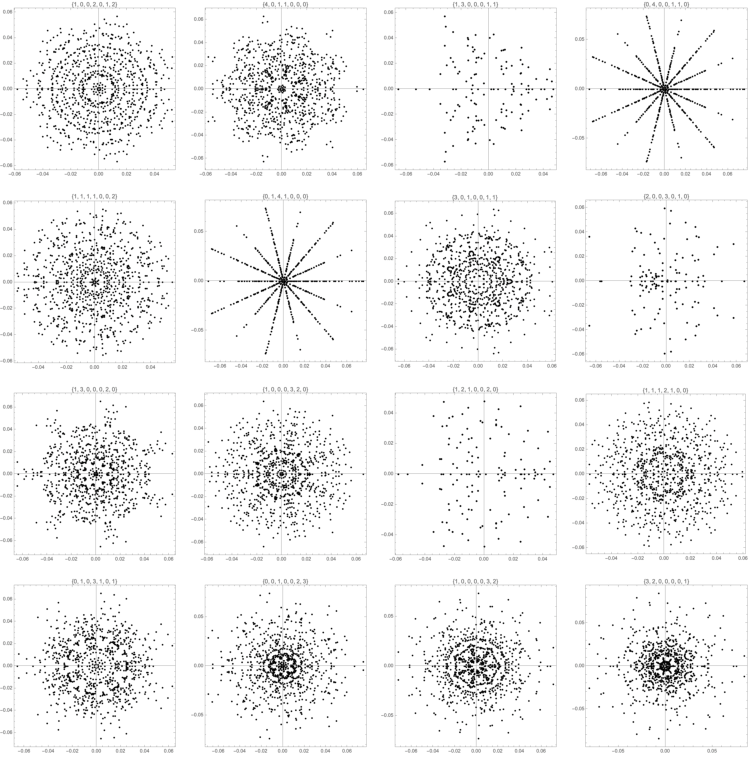
\includegraphics{figures/Mandalas.pdf}
  \caption{\label{fig:mandalas} Plots for various input histograms of the complex amplitudes of each output histogram. $N$ = 6, $m = 7$. }
\end{figure}

Further simulation suggests the following points:

\begin{itemize}
  \item There are families of histograms that give similar pictures.
  \item Most exhibit $m$-fold symmetry.
  \item Some less common families only exhibit $2$-fold symmetries.
\end{itemize}

We can investigate this using equation \ref{exp}. First we write the simplified expression for the specific unitary:

\begin{align*}
  \Ufou^{Q} &= \prod_{0 \leq i,j < m} \omega^{i \cdot j \cdot Q_{i,j}} \\
  &= \omega^{\sum_{0 \leq  i,j < m} i \cdot j \cdot Q_{i,j} \mod m}
\end{align*}

We are ready to study the simmetries. Let us fix an imput histogram: $ \vec{n} = (n_1,\cdots,n_{m})$. We consider an action of the dihedral group on this histogram. Recall that the dihedral group $D_{m}$ is the group of symmetries of a regular $m$-gon under rotations and reflections. It has the following presentation:

\[D_{m} = <r, s | s^{2} = \epsilon, srs = r^{-1}>\]

Where $r$ represents a unit rotation and $s$ a reflection. This group can acts on our histogram in the following way:

\begin{align*}
  r.(n_1, n_2, \cdots, n_{m}) &= (n_{m}, n_{1}, \cdots, n_{m-1}) \\
  s.(n_1, n_2, \cdots, n_{m}) &= (n_{m}, \cdots, n_{2}, n_{1}) \\
\end{align*}

Let us study the amplitude of output $\vec{n'}$ for a rotation: We notice that the matrices $Q$ that are compatible with $r.\vec{n}$ and $\vec{n'}$ are exactly the ones compatible with $\vec{n}$ and $\vec{n'}$ but with the lines rotated downwards, i.e. if we count the indices modulo $m$:

\begin{align*}
   \mathcal{A}_{\Ufou}(\vec{n'}, r.\vec{n}) &=  \sqrt{r.\vec{n}! \vec{n'}!} \sum_{Q \in \comp(r.\vec{n}, \vec{n'})} \frac{\omega^{\sum_{0 \leq  i,j < m} i \cdot j \cdot Q_{i,j}}}{Q!}\\
  &= \sqrt{\vec{n}! \vec{n'}!} \sum_{Q \in \comp(r.\vec{n}, \vec{n'})} \frac{\omega^{\sum_{0 \leq  i,j < m} i \cdot j \cdot Q_{i,j}}}{Q!}\\
  &= \sqrt{\vec{n}! \vec{n'}!} \sum_{Q \in \comp(\vec{n}, \vec{n'})} \frac{\omega^{\sum_{0 \leq  i,j < m} i \cdot j \cdot Q_{i,j+1}}}{Q!}\\
  &= \sqrt{\vec{n}! \vec{n'}!} \sum_{Q \in \comp(\vec{n}, \vec{n'})} \frac{\omega^{\sum_{0 \leq  i,j < m} i \cdot (j-1) \cdot Q_{i,j}}}{Q!}\\
  &= \sqrt{\vec{n}! \vec{n'}!} \sum_{Q \in \comp(\vec{n}, \vec{n'})} \frac{\omega^{\sum_{0 \leq  i,j < m} i \cdot j \cdot Q_{i,j}}\cdot \omega^{\sum_{0 \leq i,j < m} i Q_{i,j}}}{Q!}\\
  &= \sqrt{\vec{n}! \vec{n'}!} \sum_{Q \in \comp(\vec{n}, \vec{n'})} \frac{\omega^{\sum_{0 \leq  i,j < m} i \cdot j \cdot Q_{i,j}}\cdot \omega^{\sum_{0 \leq i < m} i n'_{i+1}}}{Q!}\\
  &= \omega^{\weight(\vec{n'})} \mathcal{A}_{\Ufou}(\vec{n'}, \vec{n})
\end{align*}

Where we define the weight of a histogram:\change{Maybe index from 0 everywhere}

\[\weight(\vec{n}) = 0 \cdot n_{1} + 1 \cdot n_{2} + \cdots + (m-1) \cdot n_{m-1} \mod m \]

The same type of cumputation gives:

\begin{align*}
  \mathcal{A}_{\Ufou}(\vec{n'}, s.\vec{n})   &= \omega^{\weight(\vec{n'})} \overline{\mathcal{A}_{\Ufou}(\vec{n'}, \vec{n})}
\end{align*}

This explains the plot families: within a given orbit of dihedral permutations, two input histograms will produce the exact same set of amplitudes, each shifted by a phase that depends on the weight of the corresponding \emph{output} histogram (and/or reversed along the real axis). The plots are then similar in that each of the $m$ weight classes gets shifted around by the same phase \ref{fig:weights}):\illustration{Would be nice to print the weight of each color}

\begin{figure}[ht]
  \centering
  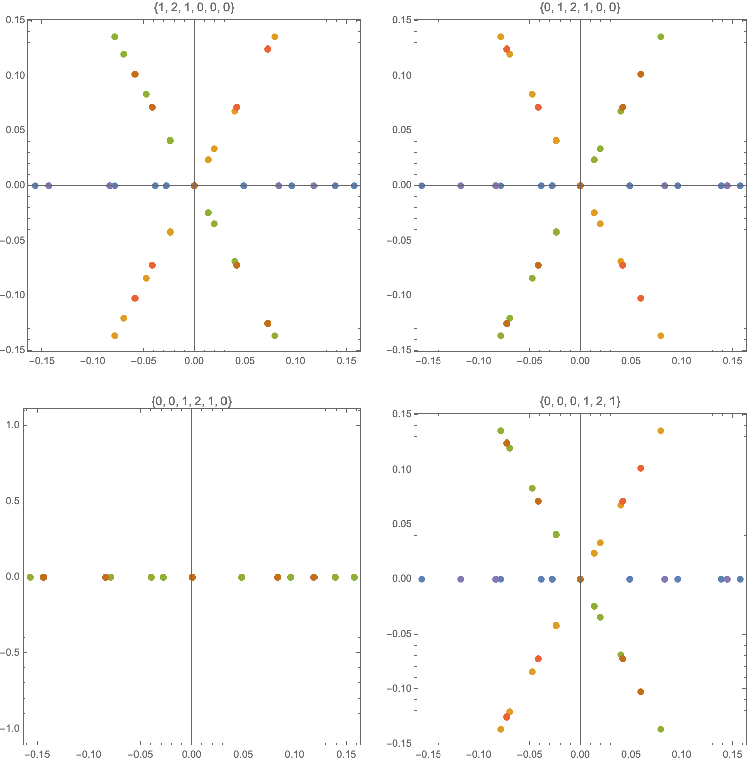
\includegraphics[scale=0.7]{figures/weights.pdf}
  \caption{\label{fig:weights} Here $N=4$, $m=6$, after each rotation the weight classes (each of a different color) get shifted by their own phase.}.
\end{figure}

We can also notice that the same reasonning applies to the output histogram:

\begin{empheq}[left = \empheqlbrace]{align*}
  \mathcal{A}_{\Ufou}(r.\vec{n'}, \vec{n})   &= \omega^{\weight(\vec{n})} \mathcal{A}_{\Ufou}(\vec{n'}, \vec{n}) \\
  \mathcal{A}_{\Ufou}(s.\vec{n'}, \vec{n})   &= \omega^{\weight(\vec{n})} \overline{\mathcal{A}_{\Ufou}(\vec{n'}, \vec{n})}
\end{empheq}

Which explains the presence of symmetries: most of the histograms studied have $m$-fold symmetry because in general the $m$ weight classes are evenly rotated, though in some cases (like the bottom left in \ref{fig:weights}) their phases line up and generate a pattern that looks sparser and less symmetric: many points overlap.


\section{Studying  the symmetries}

\section{Studying  the histogram orbits}

We've seen that the action of $D_{m}$ results in many simmetries in the fourrier transform of the histograms. Studying the corresponding permutation representation, we can analyse the situation deeper.

\subsection{Charcaters of our permutation representation of $D_{m}$}

The histograms $\hist_{N,m}$ correspond to Fock basis states for $N$ particles and $m$ ports, and induce $(V^{\hist_{N,m}},\rho)$ the permutation representation of $D_{m}$ on $\hist_{N,m}$. Let us compute its character $\chi$. Every matrix being a permutation matrix, its trace is the sum of the $1$'s on the diagonal, i.e.\ the number of fixed points of the corresponding permutation. The group $D_{m}$ has known conjugacy classes \cite{dirreps}, we compute the character for each one.

\paragraph{$\chi(r^{k})$:} Let $g = k \wedge m$ and $m = gq$. We count the histograms that verify:

\[\forall i \in \mathbb{Z}_{m}: n_{i} = n_{i+k}\]\illustration{example on unit circle}

There are $g$ orbits of size $q$, which must each be populated by a given value. These values when multiplied by $q$ must therefor equal $n$. So if $q \nmid n$ there are $0$ possibilities. If $lq = n$ there are $\E{g}{l}$ possibilities.

% \paragraph{$\chi(r)$:} We need $(n_0, n_1,\cdots, n_{m-1}) = (n_{m-1}, n_0, \cdots, n_{m-2})$:

% \[\forall i \in \mathbb{Z}_{m}: n_{i} = n_{i+1}\]

% This leads to $n_0 = \cdots = n_{m-1}$, a uniform histogram only possible if $m | n$, in which case there is $1$ possibility. Otherwise there are $0$.

\paragraph{$\chi(s)$:}

We are essentially counting the palindromes within $\hist_{N,m}$. Depending on wether $m$ is even or odd, the histogram must be in two symmetric parts with or without an extra central value.


\begin{itemize}
\item \textbf{For $m$ even and $n$ odd} palindromes are impossible because the two parts of the histogram must have the same sum.
\item \textbf{For $m = 2\tilde{m}$ and $N = 2\tilde{N}$} we have any choice for the first half of the histogram and that choice determines the second so there are $\E{\tilde{m}}{\tilde{n}}$.
\item \textbf{For $m = 2\tilde{m} + 1$ and $N = 2\tilde{N}$} we have any even choice for the middle value $i$ and any remaining choice for the first half: $\sum_{i=0}^{\tilde{n}} \E{\tilde{m}}{\tilde{n} - i} = \frac{\tilde{m} + \tilde{n}}{\tilde{n}} \E{\tilde{m}}{\tilde{n}}$.
\item \textbf{For $m = 2\tilde{m} + 1$ and $N = 2\tilde{N} + 1$} the situation is the same, this time $i$ must be odd to cancel out the extra particle: $\sum_{i=0}^{\tilde{n}} \E{\tilde{m}}{\tilde{n} - i} = \frac{\tilde{m} + \tilde{n}}{\tilde{n}} \E{\tilde{m}}{\tilde{n}}$.
\end{itemize}

Finally when $m$ is even we also need to consider the class $sr$:

\paragraph{$\chi(sr)$:} We want $(n_0,n_1,\cdots,n_{m-1}) = (n_{m-2},\cdots, n_{0}, n_{m-1})$, i.e.\ the last value $n_{m-1} = i$ is conserved and the rest must be a palindrome of odd size, and of sum (n-i).

\[\sum_{i=0}^{n} =\]\unsure{calculate this}

\subsection{Decomposing into irreducible representations}

The character table of $D_{m}$ depends on the parity of $m$:

\begin{table}
  \begin{subtable}{0.5\linewidth}
    \resizebox{\linewidth}{!}{%
    \begin{tabular}{||c | c c c c c||}
  \hline
  \multicolumn{6}{|c|}{$D_{m}$ (odd)} \\
  \hline
  conjugacy class   & $r^0$ & $r^1$ & $\cdots$ & $r^{\tilde{m}}$    & $s$ \\
  multiplicity      & 1     & 2     & 2        & 2                & $m$ \\
\hline \hline
  $\chi_{1,1}$       & 1     & 1     & $\cdots$ & 1                & 1 \\
  $\chi_{1,2}$       & 1     & 1     & $\cdots$ & 1                & (-1) \\
  $\chi_{2,k}$       & 2          & $2 \cos(\frac{2 k \pi}{m})$ & $\cdots$ & $2 \cos(\frac{2 k \tilde{m} \pi}{m})$ & 0 \\
\hline
    \end{tabular}
}

  \end{subtable}
  \begin{subtable}{0.6\linewidth}

    \resizebox{\linewidth}{!}{%
    \begin{tabular}{||c | c c c c c c||}
  \hline
  \multicolumn{7}{|c|}{$D_{m}$ (even)} \\
  \hline
  conjugacy class   & $r^0$     & $r^1$             & $\cdots$    & $r^{\tilde{m}}$      & $s$         & $sr$\\
  multiplicity      & 1         & 2                 & 2           & 1                  & $\tilde{m}$ & $\tilde{m}$\\
\hline \hline
  $\chi_{1,1}$       & 1         & 1                 & $\cdots$    & 1                 & 1             & 1 \\
  $\chi_{1,2}$       & 1         & (-1)              & $\cdots$    & ${(-1)}^{\tilde{m}}$  & 1             & (-1)\\
  $\chi_{1,3}$       & 1         & 1                 & $\cdots$    & 1                 & (-1)          & (-1) \\
  $\chi_{1,4}$       & 1         & (-1)              & $\cdots$    & ${(-1)}^{\tilde{m}}$  & (-1)          & 1\\
  $\chi_{2,k}$       & 2         & $2 \cos(\frac{2 k \pi}{m})$ & $\cdots$ & $2 \cos(\frac{2 k \tilde{m} \pi}{m})$ & 0 & 0\\
\hline
    \end{tabular}
}
  \end{subtable}
\end{table}

\subsection{Decomposing translationally invariant unitaries}

Let us consider a translationally invariant unitary $U$, that is $U$ has eigenvectors:

\[U \ket{n_{\theta}} = e^{i\phi(\theta)} \ket{\theta}\]

Then we can use the following decomposition:

\begin{align*}
  \bra{\vec{x}} U \ket{\vec{y}} &= \sum_{\theta}\braket{\vec{x}}{\vec{n_{\theta}}} U \braket{\vec{n_{\theta}}}{\vec{y}}  \\
   &= \sum_{\theta}\braket{\vec{x}}{\vec{n_{\theta}}} \braket{\vec{n_{\theta}}}{\vec{y}} e^{i \phi(\theta)}
\end{align*}


\section{Asymptotics of bosonic amplitudes for compatible histograms}

In this part $U$ is an arbitrary unitary. We consider vectors of amplitudes $\vec{\nu}$ and phases $\vec{\phi}$ in $\mathbb{R}^{m}$ such that the following quantum state is well defined:

\[\ket{\psiVec{\nu}{\phi}} = \sum_{i = 1}^{m} \sqrt{\nu_{i}} e^{\phi_{i}} \ket{i} \]

\begin{definition}[Compatibility]
  We say that $\vec{\nu}, $ and $\vec{\nu'}$ are compatible under the unitary $U$ if there exists $\vec{\phi}$ and $\vec{\phi'}$ such that:

  \[\ket{\psiVec{\nu'}{\phi'}} = U \ket{\psiVec{\nu}{\phi}}\]
\end{definition}\illustration{3D example with cones}

Note that this is equivalent to:

\[\Braket{\psiVec{\nu'}{\phi'} | U | \psiVec{\nu}{\phi}} = 1\]

\begin{prop}
  The fock state $\ket{\vec{n}}$ can have the following formula for any arbirtary $\vec{\nu}$:
  \[\ket{\vec{n}} = c \int \frac{d^{m}\vec{\phi}}{(2\pi)^{m}} e^{-i \vec{\phi} \cdot \vec{n}} \ket{\psiVec{\nu}{\phi}}^{\otimes n}\]
where:

\[c_{\vec{\nu},\vec{n}} := \frac{1}{\prod_{i} \sqrt{\nu_{i}}^{n_{i}} \sqrt{\frac{n!}{\prod_{i} n_{i}}}} \]
\end{prop}

Note that when $\nu_{i} = \frac{n_i}{n}$, Stirling's formula ensures that $c$ decreases polynomially in $n$.\change{add proof somewhere}

From now on we will consider two compatible histograms:

\[\begin{cases}
    \vec{n} = n \cdot \vec{\nu} \\
    \vec{n'} = n \cdot \vec{\nu'}
  \end{cases}\]

We denote:

\[\Ampl{\vec{n}}{\vec{n'}} = \frac{\bra{\vec{n'}} U \ket{\vec{n}}}{c_{\vec{n}, \vec{\nu}} c_{\vec{n}, \vec{\nu}}}\]

We then have:

\[\Ampl{\vec{n}}{\vec{n'}} =  \int \frac{d^{m}\vec{\phi}}{{(2\pi)}^{m}} \frac{d^{m}\vec{\phi'}}{{(2\pi)}^{m}} {\left[ \Braket{\psiVec{\nu'}{\phi'} | U | \psiVec{\nu}{\phi}} e^{-i \vec{\phi} \cdot \vec{\nu} + i \vec{\phi'} \cdot \vec{\nu'}} \right] }^{\otimes n} \]

Since $\vec{\nu}$ and $\vec{\nu'}$ are compatible, there exists phase vectors for witch the bracket term will be of norm $1$, we will show that the amplitude will be dominated by those contributions.

\subsection{Factoring out common phases}

We notice that the integral is stable under phase vector translations. This motivates an attempt to equalise both first components of the two phase vectors.  We let:

\[\undertilde{\vec{\phi}} = \begin{pmatrix}
                              0 \\
                              \phi_{2} - \phi_{1} \\
                              \vdots \\
                              \phi_{m} - \phi_{1}
                            \end{pmatrix}
                            ; \ \undertilde{\vec{\phi'}} = \begin{pmatrix}
                              0 \\
                              \phi'_{2} - \phi'_{1} \\
                              \vdots \\
                              \phi'_{m} - \phi'_{1}
                            \end{pmatrix}
                          \]

Rewriting the bracket term in the amplitude integral gives us the following:\change{put this in an appendix}

\begin{align*}
  \braKet{\psiVec{\nu'}{\phi'}}{U}{\psiVec{\nu}{\phi}} e^{-i \vec{\phi} \cdot \vec{\nu} + i \vec{\phi'} \cdot \vec{\nu'}} &= \left(\sum_{j} \sqrt{\nu'_{j}} e^{i \undertilde{\phi'}_{j} + i\phi'_{1}} \bra{j}  \right) U \ket{\psiVec{\nu}{\phi}} e^{-i \vec{\phi} \cdot \vec{\nu} + i \vec{\phi'} \cdot \vec{\nu'}} \\
                                                                                                                             &= e^{-i\phi'_{1}} \braKet{\psiVec{\nu'} {\undertilde{\phi'}}}{U}{\psiVec{\nu}{\phi}} e^{-i \vec{\phi} \cdot \vec{\nu} + i \vec{\phi'} \cdot \vec{\nu'}} \\
                                                                                                                             &= e^{-i\phi'_{1} + i \phi_{1}} \braKet{\psiVec{\nu'}{\undertilde{\phi'}}}{U}{\psiVec{\nu}{\undertilde{\phi}}} e^{-i \vec{\phi} \cdot \vec{\nu} + i \vec{\phi'} \cdot \vec{\nu'}} \\
                                                                                                                             &= e^{-i\phi'_{1} + i \phi_{1}} \braKet{\psiVec{\nu'} {\undertilde{\phi'}}}{U}{\psiVec{\nu}{\undertilde{\phi}}} e^{-i \left(\sum_{j} \nu_{j}(\undertilde{\phi}_{j} + \phi_{1}) \right) + i \vec{\phi'} \cdot \vec{\nu'}} \\
                                                                                                                             &= e^{-i\phi'_{1} + i \phi_{1}} \braKet{\psiVec{\nu'} {\undertilde{\phi'}}}{U}{\psiVec{\nu}{\undertilde{\phi}}} e^{-i \left( \sum_{j} \nu_{j} \phi_{1} + \sum_{j} \nu_{j}\undertilde{\phi}_{j} \right) + i \vec{\phi'} \cdot \vec{\nu'}} \\
                                                                                                                             &= e^{-i\phi'_{1} + i \phi_{1} -i \phi_{1} \sum_{j} \nu_{j}} \braKet{\psiVec{\nu'} {\undertilde{\phi'}}}{U}{\psiVec{\nu}{\undertilde{\phi}}} e^{-i \vec{\undertilde{\phi}} \cdot \vec{\nu} + i \vec{\phi'} \cdot \vec{\nu'}} \\
                                                                                                                             &= e^{-i\phi'_{1} + i \phi_{1} -i \phi_{1} \sum_{j} \nu_{j} +i \phi'_{1} \sum_{j} \nu'_{j}} \braKet{\psiVec{\nu'} {\undertilde{\phi'}}}{U}{\psiVec{\nu}{\undertilde{\phi}}} e^{-i \vec{\undertilde{\phi}} \cdot \vec{\nu} + i \vec{\undertilde{\phi'}} \cdot \vec{\nu'}} \\
\end{align*}


In the last line the first phase term is $1$ because the $\nu_{i}$'s sum to unity. Therefor:

\[ \Ampl{\vec{n}}{\vec{n'}} =  \int \frac{d \phi_{1}}{2\pi} \frac{d \phi'_{1}}{2\pi} \int \frac{d^{m-1}\vec{\undertilde{\phi}}}{{(2\pi)}^{m-1}} \frac{d^{m-1}\vec{\undertilde{\phi'}}}{{(2\pi)}^{m-1}} {\left[ \Braket{\psiVec{\nu'}{\undertilde{\phi'}} | U | \psiVec{\nu}{\undertilde{\phi}}} e^{-i \vec{\undertilde{\phi}} \cdot \vec{\nu} + i \vec{\undertilde{\phi'}} \cdot \vec{\nu'}} \right] }^{\otimes n}  \]

So dropping the tildes and assuming $\phi_{1} = \phi'_{1} = 0$ we have:

\[ \Ampl{\vec{n}}{\vec{n'}} =  \int \frac{d^{m-1}\vec{\phi}}{{(2\pi)}^{m-1}} \frac{d^{m-1}\vec{\phi'}}{{(2\pi)}^{m-1}} {\left[ \Braket{\psiVec{\nu'}{\phi'} | U | \psiVec{\nu}{\phi}} e^{-i \vec{\phi} \cdot \vec{\nu} + i \vec{\phi'} \cdot \vec{\nu'}} \right] }^{\otimes n}  \]

\subsection{Stationnary phase conditions}

To obtain an approximation, we want to apply the stationary phase method. The idea is that for complex integrands whose phase rotates rapidly, the corresponding amplitudes will tend to cancel out. The main contribution then comes from the points where the phase shifts slowly. We show that this happens exactly at the points that realise compatibility for $\vec{\nu}$ and $\vec{\nu}$. Let us rewrite the amplitude:

\[ \Ampl{\vec{n}}{\vec{n'}} =  \int \frac{d^{m-1}\vec{\phi}}{{(2\pi)}^{m-1}} \frac{d^{m-1}\vec{\phi'}}{{(2\pi)}^{m-1}} e^{n g(\vec{\phi}, \vec{\phi'})}  \]

Where:

\[g(\check{\phi}, \vec{\phi'}) := -i \vec{\phi} \cdot \vec{\nu} + i \vec{\phi'} \cdot \vec{\nu'} + \ln  \bra{\psi_{\vec{\nu'}\vec{\phi'}}} U \ket{\psiVec{\nu}{\phi}} \]

Let us examin the conditions for $\nabla_{\phi} g = \nabla_{\phi'} g = 0$. We want to show that the phases that satisfy this are exactly the ones that realise compatibility. The reciprocal is quite obvious, one can verify it by looking at the expresssion for the derivatives in the following lines and replace the terms respecting compatibility. We show the direct implication:


\begin{align*}
  \nabla_{\phi} g = 0 &\\
  &\implies -i \nu_{j} + \frac{i \Braket{\psiVec{\nu'}{\phi'} | U | j} \braket{j}{\psiVec{\nu}{\phi}}}{\Braket{\psiVec{\nu'}{\phi'} | U | \psiVec{\nu}{\phi}}} = 0 \; \; \; (\forall j > 1) \\
  &\implies \Braket{\psiVec{\nu'}{\phi'} | U | j} = \Braket{\psiVec{\nu'}{\phi'} | U | \psiVec{\nu}{\phi}} \cdot \sqrt{\nu_{j}} e^{-i \phi_{j}}
\end{align*}

Doing the same for $\nabla_{\phi'} g$ we get the two conditions for all $j > 1$:

\begin{empheq}[left = \empheqlbrace]{align}
\Braket{\psiVec{\nu'}{\phi'} | U | j} &= \Lambda \sqrt{\nu_{j}} e^{i \phi_{j}}\label{stat:1} \\
\Braket{j | U | \psiVec{\nu}{\phi}} &= \Lambda \sqrt{\nu'_{j}} e^{i \phi'_{j}}\label{stat:2}
\end{empheq}

where:
\[\Lambda := \Braket{\psiVec{\nu'}{\phi'} | U | \psiVec{\nu}{\phi}}\]

Now we need only show that whenever \ref{stat:1} and \ref{stat:2} are verified, then $|\Lambda| = 1$:

\begin{align*}
  \Lambda &= \sum_{j} \braket{\psiVec{\nu'}{\phi'}}{j} \Braket{j | U | \psiVec{\nu}{\phi}} \\
  &= \sum_{j} \sqrt{\nu'_{j}} e^{-i \phi'^{j}} \Braket{j | U | \psiVec{\nu}{\phi}} \\
          &\stackrel{\ref{stat:2}}{=} \sqrt{\nu'_{1}} \Braket{1 | U | \psiVec{\nu}{\phi}} + \sum_{j>1} \nu'_{j} \Lambda \\
            &= \sqrt{\nu'_{1}} \Braket{1 | U | \psiVec{\nu}{\phi}} + \Lambda (1 - \nu'_{1}) \\
  \implies \sqrt{\nu'_{1}}\Lambda &=  \Braket{1 | U | \psiVec{\nu}{\phi}}
\end{align*}

We can apply the same reasoning using \ref{stat:1} to obtain:

\begin{empheq}[left = \empheqlbrace]{align*}
\bra{\psiVec{\nu'}{\phi'}} U &= \Lambda \bra{\psiVec{\nu}{\phi}} \\
U \ket{\psiVec{\nu}{\phi}} &= \Lambda \ket{\psiVec{\nu'}{\phi'}}
\end{empheq}

So $|\Lambda| = 1$.

\subsection{Gaussian expansion}

In this part we expand $g$ into its taylor series around these crytical points realising compatibility. We then plug the expansion into the amplitude integral to obtain an asymoptotic formula. We let the family of solutions be indexed by $\alpha$:

\[\nabla_{\phi}g(\phi_{\alpha},\phi'_{\alpha}) = \nabla_{\phi'}g(\phi_{\alpha},\phi'_{\alpha}) = 0\]

At the second order we get:

\[g(\phi,\phi') = g_{\alpha} - \frac{1}{2} \vec{\delta}^{T} \Gamma_{\alpha} \vec{\delta} + O(\vec{\delta})\]

\begin{empheq}[left = \empheqlbrace]{align*}
g_{\alpha} &= \Braket{\psiVec{\nu}{\phi_{\alpha}} | U | \psiVec{\nu'}{\phi'_{\alpha}}} - \vec{\phi_{\alpha}} \cdot \vec{\nu} + \vec{\phi'_{\alpha}} \cdot \vec{\nu'} \\
\vec{\delta} &= (\phi - \phi_{\alpha}, \phi' - \phi'_{\alpha})^{T} \\
\Gamma_{\alpha} &= -\begin{pmatrix}
\nabla_{\phi}\nabla_{\phi}g & \nabla_{\phi}\nabla_{\phi'}g \\
\nabla_{\phi}\nabla_{\phi'}g & \nabla_{\phi'}\nabla_{\phi'}g
\end{pmatrix}_{\alpha} \\
\end{empheq}

Then:

\begin{align*}
  \Ampl{\vec{n}}{\vec{n'}} &\sim \sum_{\alpha} \frac{e^{i n g_{\alpha}}}{(2 \pi)^{2(m-1)}} \int d \phi^{m-1} d \phi'^{m-1} e^{-\frac{n}{2} \vec{\delta}^{T} \Gamma_{\alpha} \vec{\delta}} \\
  &\sim \sum_{\alpha} \frac{e^{in g_{\alpha}}}{(2 \pi)^{2(m-1)}} \frac{1}{\sqrt{\det(\Gamma_{\alpha})}}
\end{align*}

Now recall the normalisation term, to which we give an equivalent as $n \to \infty$ using Stirling's formula:

\begin{align*}
  c_{\vec{\nu}, \vec{n}} &= \frac{1}{\sqrt{\frac{n!}{\prod_{i} n_{i}!}} \prod_{i} \sqrt{\nu_{i}}^{n_{i}}} \\
                           &= \sqrt{\frac{n^{n}}{n!} \prod_{i} \frac{n_{i}!}{n_{i}^{n_{i}}}}\\
                         &\sim \sqrt{\frac{1}{\sqrt{2 \pi n}} \prod_{i} \sqrt{2 \pi n_{i}}} \\
  &\sim (2 \pi n)^{\frac{m-1}{4}} \prod_{i} \nu_{i}^{\frac{1}{4}}
\end{align*}

Finally, taking into account both of the terms:\change{maybe cite equation}

\begin{gather}
  \Braket{\vec{n'} | U | \vec{n}} \sim \frac{1}{(2 \pi n)^{\frac{m-1}{2}}} \sum_{\alpha} \sqrt{\frac{\prod_{i} \sqrt{\nu_{i} \nu'_{i}}}{\det \Gamma_{\alpha}}} e^{i n g_{\alpha}}\label{asympt:1}
\end{gather}

\subsection{Closer look at the Hessian}

Looking at the derivatives of $g$ one can get a formula for each coefficient of the Hessian:

\begin{align*}
  -\Gamma_{\phi_{i}, \phi_{j}} &= \frac{\partial^{2} g}{\partial \phi_{i} \partial \phi_{j}} \\
  &= i \frac{\partial}{\partial \phi_{j}} \frac{\Braket{\psiVec{\nu'}{\phi'} | U \Pi_{i} | \psiVec{\nu}{\phi}}}{\Braket{\psiVec{\nu'}{\phi'} | U | \psiVec{\nu}{\phi}}} \\
  &= -\delta_{i,j} \frac{\Braket{\psiVec{\nu'}{\phi'} | U \Pi_{i} | \psiVec{\nu}{\phi}}}{\Braket{\psiVec{\nu'}{\phi'} | U | \psiVec{\nu}{\phi}}} + \frac{\Braket{\psiVec{\nu'}{\phi'} | U \Pi_{i} | \psiVec{\nu}{\phi}} \Braket{\psiVec{\nu'}{\phi'} | U \Pi_{j} | \psiVec{\nu}{\phi}}}{\Braket{\psiVec{\nu'}{\phi'} | U | \psiVec{\nu}{\phi}}^{2}} \\
&= -\delta_{i;j}\nu_{i} + \nu_{i}\nu_{j}
\end{align*}

Similar computations for the other indices give us the following set of formulas:

\begin{empheq}[left = \empheqlbrace]{align*}
-\Gamma_{\phi_{i}, \phi_{j}} &= -\delta_{i,j} \nu_{i} + \nu_{i} \nu_{j} \\
-\Gamma_{\phi'_{i}, \phi'_{j}} &= -\delta_{i,j} \nu'_{i} + \nu'_{i} \nu'_{j} \\
-\Gamma_{\phi'_{i}, \phi_{j}} &= U_{i,j} \sqrt{\nu'_{i} \nu_{j}} e^{\phi_{j} - \phi'_{i} - \Lambda} - \nu'_{i} \nu_{j}
\end{empheq}

\newpage
\listoftodos[Notes]

\end{document}
